\chapter{Supernova Model Evidence Extractor}
\label{chp:SMEE}

The Supernova Model Evidence Extractor (SMEE) is a parameter estimation tool for GWs from CCSNe. It performs Bayesian model selection to make classification statements about an observed waveform. Due to the inherently random nature of CCSN waveforms, we decompose a catalog of related waveforms into principal components (PCs) that contain the most prominent features of a catalog. These PCs are then used to produce waveform reconstructions and perform model selection. Our waveforms and PCs are in the form of real-valued ASD spectrograms and depend only on the time and frequency of GW emission in order to be as robust as possible against the stochastic nature of CCSN signals. This chapter will explain the methodology and inner workings behind SMEE's algorithm.

\section{Bayesian Inference}

Bayesian Inference is a powerful analysis technique that has become common in astrophysics and other fields. It allows for the comparison of hypotheses while continuously accounting for new data. Bayes theorem can be thought of as relating the probability that a hypothesis is true to the more useful probability that our measured data would be observed given that the hypothesis is true~\cite{thesis_josh}. Explicitly, 
\begin{equation}
\label{equ:Bayes}
    p(H|D) = \frac{p(H)p(D|H)}{p(D)}
\end{equation}
where $p(H|D)$ is the posterior probability, $p(H)$ is the prior probability, $p(D|H)$ is the model evidence, and $p(D)$ is the probability of obtaining the data $D$ independently of the hypothesis, also called a marginal probability. The posterior probability represents what we know about a hypotheses after considering all of the data and previously known information. It is commonly the final desired result of probability calculations. The prior probability represents what is known about the hypothesis before considering the data. For many situations involving supernovae it is common to make as few assumptions as possible, meaning that some parameter prior distributions are frequently flat or constant across a given parameter space. The model evidence, $p(D|H)$, tells us how well the observed data agrees with what we would expect given our model to be true. This is the most important term for model selection.

When two hypotheses, or models, need to be compared to each other, it useful to take a ratio of their posterior probabilities. This is known as an odds ratio~\cite{thesis_josh, thesis_jade},
\begin{equation}
\label{equ:Odds}
    O_{ij} = \frac{p(M_{i}|D)}{p(M_{j}|D)} = \frac{p(M_{i})p(D|M_{i})}{p(M_{j})p(D|M_{j})} = \frac{p(M_{i})}{p(M_{j})}B_{ij}
\end{equation}
where $B_{ij}$ is a Bayes factor defined as the ratio of model evidences,
\begin{equation}
    B_{ij} = \frac{p(D|M_{i})}{p(D|M_{j})}
\end{equation}
It's worth noting that when we plug equation \ref{equ:Bayes} into our odds ratio the denominator factors out as it is the same for each model. If neither model is preferred a priori, then $p(M_{i}) = p(M_{j})$ and the odds ratio simplifies to a Bayes factor. This Bayes factor is the primary output of a model selection algorithm such as SMEE. For a model defined by a set of parameters, the model evidence, $Z$, can be calculated by integrating the likelihood, $p(D|\theta,M)$, multiplied by the prior, $p(\theta|M)$, across all parameter values $\theta$,
\begin{equation}
\label{equ:evidence_def}
    Z = p(D|M) = \int_{\theta} p(\theta|M)p(D|\theta,M)d\theta
\end{equation}
This integral is commonly difficult or impossible to solve analytically, leading to the use of numerical techniques such as nested sampling~\cite{thesis_josh, thesis_jade, logue:12, powell:16b, 2017PhRvD..96l3013P}.

\section{Power Spectral Density and Likelihood}

Our statistics depend on the power of GW emission in a frequency bin. Specifically, we calculate the power spectral density for each tile in our spectrograms. The two-sided PSD is defined~\cite{miller2012probability}, 
\begin{equation}
\label{equ:PSD_def}
    S_{xx}(f) = \lim_{T \to \infty} \left\langle |\tilde{d}(f)|^{2} \right\rangle
\end{equation}
where the brackets indicate an expectation value and $\tilde{d}(f)$ is a Fourier transform of detector data defined as,
\begin{equation}
    \tilde{d}(f) = \frac{1}{\sqrt{T}} \int_{0}^{T} d(t)e^{-2\pi it}dt
\end{equation}
Technically, SMEE approximates a PSD by calculating a periodogram at each time in the spectrogram. Essentially this means that there is no infinite limit or averaging in equation \ref{equ:PSD_def}\,. The accuracy of our PSDs with respect to random detector noise could be improved by averaging over more time, but this also lowers signal amplitudes and offered no performance improvement in our testing. Rewriting equation \ref{equ:PSD_def} gives,
\begin{equation}
\label{equ:PSD_approx}
    S_{xx}(f) \approx |\tilde{d}(f)|^{2} = \mathbb{R}[\tilde{d}(f)]^{2} + \mathbb{I}[\tilde{d}(f)]^{2}
\end{equation}
where $\mathbb{R}$ and $\mathbb{I}$ represent the real and imaginary parts of the Fourier transform respectively. Equation \ref{equ:PSD_approx} shows explicitly that our PSD approximation is a sum of two squared numbers. For Gaussian noise it can be shown that these will both be Gaussian variables. Detector data can be written as the linear sum of Gaussian noise and a GW signal~\cite{veitch:15},
\begin{equation}
\label{equ:d_def}
    \tilde{d}(f) = \tilde{n}(f) + \tilde{h}(f)
\end{equation}
For Gaussian noise,
\begin{equation}
\label{equ:gaus_noise}
    \left\langle \tilde{n}(f) \right\rangle = 0 \quad\text{and}\quad \left\langle |\tilde{n}(f)|^{2} \right\rangle = \sigma_{f}^{2} = \frac{S(f)}{2}
\end{equation}
where $S(f)$ is the one-sided noise spectral density. The leftmost equality tells us that the expectation value of the detector data Fourier transform is equal to the Fourier transform of the signal.
\begin{equation}
\label{equ:d_mean}
    \left\langle \tilde{d}(f) \right\rangle = \tilde{h}(f) %\quad\text{and}\quad \left\langle |\tilde{d}(f)|^{2} \right\rangle = |\tilde{h}(f)|^{2}
\end{equation}
Looking back at equation \ref{equ:PSD_approx}, the right-hand side is the sum of two squared Gaussian variables. Each variable has a mean determined by the signal (as seen in equation \ref{equ:d_mean}) and a variance determined by the detector noise (right-hand side of equation \ref{equ:gaus_noise}). If these were Gaussian variables with unit variance then this would resemble a noncentral chi-squared distribution with two degrees of freedom. In order to obtain unit variance, we must divide our variables by their current variance. The right side of equation \ref{equ:gaus_noise} tells us the variance for Gaussian noise. The variance of the real and imaginary parts will be half of the total variance,
\begin{equation}
    \left\langle |\tilde{n}(f)|^{2} \right\rangle = \left\langle \mathbb{R}[\tilde{n}(f)]^{2} \right\rangle + \left\langle \mathbb{I}[\tilde{n}(f)]^{2} \right\rangle
\end{equation}
This gives us,
\begin{equation}
    \sigma^{2} = \frac{S(f)}{4}
\end{equation}
Dividing through in equation \ref{equ:PSD_approx} gives,
\begin{equation}
    \frac{S_{xx}(f)}{\sigma^{2}} \approx \frac{\mathbb{R}[\tilde{d}(f)]^{2}}{\sigma^{2}} + \frac{\mathbb{I}[\tilde{d}(f)]^{2}}{\sigma^{2}}
\end{equation}
Plugging in $\sigma^{2}$ explicitly and replacing $S_{xx}$ with the one-sided PSD of detector data $S_{x}$ (where $S_{x} = 2S_{xx}$ for real data),
\begin{equation}
    \frac{2S_{x}(f)}{S(f)} \approx \frac{4\mathbb{R}[\tilde{d}(f)]^{2}}{S(f)} + \frac{4\mathbb{I}[\tilde{d}(f)]^{2}}{S(f)}
\end{equation}
This is the final result used by SMEE. Because we now have two squared Gaussian variables each with unit variance and nonzero mean, this can be represented by a noncentral chi-squared distribution.

We can do a quick sanity check by assuming momentarily that there is no signal present, $\tilde{h}(f) = 0$, and that our data consists entirely of Gaussian noise. With no signal present, our noncentral chi-squared distribution simplifies to a standard chi-squared distribution and,
\begin{equation}
    \left\langle S_{x}(f) \right\rangle = S(f)
\end{equation}
This leads immediately to an expectation value for our chi-squared variable,
\begin{equation}
    \left\langle \frac{2S_{x}(f)}{S(f)} \right\rangle = 2
\end{equation}
For Gaussian noise, our expectation value is equal to the number of degrees of freedom. This is as expected for a chi-squared variable~\cite{stats_shao}.

\section{Noncentral Chi-Squared Distribution}

If $(X_{1}, X_{2}, ... , X_{i}, ... , X_{k})$ are $k$ independent, normally distributed random variables with means $\mu_{i}$ and unit variances, then the sum of their squares, $x$, is a noncentral chi-squared variable~\cite{freedman2007statistics}.
\begin{equation}
    x = \sum_{i=1}^{k} X_{i}^{2}
\end{equation}
The noncentrality parameter, $\lambda$, is related to the means of each variable and is defined as,
\begin{equation}
    \lambda = \sum_{i=1}^{k} \mu_{i}^{2}
\end{equation}
The full probability density function depends only on $k$ and $\lambda$ and is defined,
\begin{equation}
\label{equ:chi_pdf}
    P(x|\lambda) = \frac{1}{2}e^{-(x + \lambda) / 2}\Big(\frac{x}{\lambda}\Big)^{k/4-1/2} I_{k/2-1}(\sqrt{x\lambda})
\end{equation}
where $I_{\alpha}$ refers to a modified Bessel function of the first kind. Plugging in $k = 2$, for two degrees of freedom, gives,
\begin{equation}
    P(x|\lambda) = \frac{1}{2}e^{-(x + \lambda) / 2}\,I_{0}(\sqrt{x\lambda})
\end{equation}
This is the likelihood for a single frequency bin. For a series of data points, such as the bins within a spectrogram, the total likelihood is the product of the likelihoods for each bin. SMEE actually calculates the $\log$ of the likelihood, which means the product becomes a sum, and for $N$ data points our signal likelihood becomes,
\begin{equation}
\label{equ:signal_like_N_def}
    \log \mathcal{L}_{S} = \sum_{n=1}^{N} \left( \log(1/2) - \frac{(x_{n} + \lambda_{n})}{2} + \log\Big(I_0(\sqrt{x_{n}\lambda_{n}})\Big) \right)
\end{equation}
A subscript $n$ has been added to $x$ and $\lambda$ to indicate that they differ for each bin.

The chi-squared variable that SMEE uses was defined in the previous section.
\begin{equation}
\label{equ:x_def}
    x = \frac{2S_{x}(f)}{S(f)} \approx \frac{2\,d_{n}^{2}}{S(f)}
\end{equation}
where $S_{x}(f)$ refers to a one-sided PSD of detector data and $S(f)$ is the one-sided noise spectral density. A new notation, $d_{n}\,$, is introduced above as the periodogram approximation of a one-sided ASD of detector data ($d_{n} = |\tilde{d}(f)|$). Its subscript $n$ indicates that it represents the power of a single bin within a spectrogram. Spectrograms consist of multiple PSDs at many different times, so $d_{n}^{2}\,$, the power in each bin, is a function of both frequency and time. Going forward, however, both $f$ and $t$ will be omitted from notation for the sake of brevity and presentation. The noncentrality parameter used in SMEE is,
\begin{equation}
\label{equ:lambda_def}
    \lambda = \frac{2\,h_{n}^{2}}{S(f)}
\end{equation}
where $h_{n}$ is a one-sided ASD of the signal. Once again, the subscript $n$ indicates that it represents the power of a single bin from within a spectrogram and is therefore a function of $f$ and $t$. One quick way to arrive at this result is to consider equation \ref{equ:d_mean}\,, which tells us that $\tilde{h}(f)$ is the mean of $\tilde{d}(f)\,$. Squaring that mean and dividing by the same variance we used to obtain our chi-squared variable ($\sigma^{2} = \frac{S(f)}{4}$) gives us equation \ref{equ:lambda_def}\,. We can also arrive at this result by considering the expectation value of our chi-squared variable. To do that, I will first take the absolute square and expectation value of equation \ref{equ:d_def}\,,
\begin{equation}
\label{equ:d2_def}
    \langle |\tilde{d}(f)|^{2} \rangle = \langle |\tilde{n}(f)|^{2} \rangle + \langle |\tilde{h}(f)|^{2} \rangle
\end{equation}
There are no cross terms because we assume that $\tilde{n}(f)$ and $\tilde{h}(f)$ are entirely independent of each other and $\langle \tilde{n}(f)\tilde{h}(f) \rangle = 0$\,. Rewriting this with our simpler one-sided ASD notation,
\begin{equation}
    \left\langle d_{n}^{2} \right\rangle = \left\langle n_{n}^{2} \right\rangle + \left\langle h_{n}^{2} \right\rangle
\end{equation}
The expectation value of our chi-squared variable is then,
\begin{equation}
    \begin{split}
    \left\langle \frac{2\,d_{n}^{2}}{S(f)} \right\rangle =& \left\langle \frac{2\,n_{n}^{2}}{S(f)} \right\rangle + \left\langle \frac{2\,h_{n}^{2}}{S(f)} \right\rangle \\
    =& \,\,2 + \frac{2\,h_{n}^{2}}{S(f)} \\
    =& \,\,k + \lambda
    \end{split}
\end{equation}
This is the correct result for a noncentral chi-squared variable and shows that $\lambda$ is properly defined~\cite{stats_shao, freedman2007statistics}.

We can now plug in $x$ and $\lambda$ from equations \ref{equ:x_def} and \ref{equ:lambda_def} into equation \ref{equ:signal_like_N_def} to get our final signal model likelihood,
\begin{equation}
\label{equ:signal_like_def}
    \log \mathcal{L}_{S} = N\log(1/2) + \sum_{n=1}^{N} \left( \frac{-(d_{n}^{2} + h_{n}^{2})}{S(f)} + \log\Big(I_0(\frac{2 d_{n} h_{n}}{S(f)})\Big) \right)
\end{equation}
where $d_{n}$ and $h_{n}$ represent one-sided ASDs of the detector data and signal respectively. This likelihood value represents how well our data fits our signal hypothesis. The noise likelihood represents how well our data fits the hypothesis of pure Gaussian noise. We can obtain the noise likelihood by setting $h_{n} = 0$ in equation \ref{equ:signal_like_def}\,. This is equivalent to using the standard chi-squared distribution with $k = 2\,$. In either case, for $N$ data points we obtain a final noise likelihood of,
\begin{equation}
\label{equ:noise_like_def}
    \log \mathcal{L}_{N} = N\log(1/2) - \sum_{n=1}^{N} \frac{d_{n}^{2}}{S(f)}
\end{equation}

Equation \ref{equ:signal_like_def} contains the signal model, $h_{n}\,$. This represents the CCSN signal hypothesized to be in the data. Our signal model has the units of an ASD and is constructed out of principal components. These principal components are created from simulated CCSN waveforms and will be discussed in the next section.

\section{Principal Component Analysis}
\label{sec:PCA}

PCA is performed on a catalog of waveforms to create a set of orthogonal basis vectors called Principal Components (PCs). The PCs contain the most important features of the waveforms in a catalog~\cite{logue:12, powell:16b, 2017PhRvD..96l3013P, heng:09}. For time domain signals, each input waveform is a simple vector. The signals used in SMEE are three second long zero-padded amplitude spectral density (ASD) spectrograms. Each successive ASD in a spectrogram is a vector, containing one power value for each frequency bin. We attach data from the second ASD to the back of the first, and so on, to create a single vector out of each spectrogram. We then create an $m \times n$ matrix $\textbf{D}$, where each row contains a waveform, $m$ is the number of waveforms in the catalog, and $n$ is the length of each waveform. The covariance matrix can be defined by,
\begin{equation}
    \label{equ:covariance}
    \textbf{C} = \frac{1}{m}\textbf{D}\textbf{D}^{T}
\end{equation}
In order to obtain a set of basis vectors that span the linear space of each column in $\textbf{D}$, we would like to find the normalized eigenvectors of $\textbf{C}$. This will allow us to uniquely represent each catalog waveform as a linear combination of these eigenvectors. While $m$ is typically on the order of $\sim$ 10, $n$ is usually orders of magnitude larger. This means the above factoring can be very computationally expensive. This problem can mitigated by instead calculating the eigenvectors, $\boldsymbol\Sigma$, of $\textbf{D}^{T}\textbf{D}$ such that,
\begin{equation}
    \textbf{D}^{T}\textbf{D}\boldsymbol\Sigma_{i} = u_{i}\boldsymbol\Sigma_{i}
\end{equation}
where $u_{i}$ is the corresponding eigenvalue for each eigenvector. If we pre-multiply each side by $\textbf{D}$, then,
\begin{equation}
    \textbf{D}\textbf{D}^{T}\textbf{D}\boldsymbol\Sigma_{i} = u_{i}\textbf{D}\boldsymbol\Sigma_{i}
\end{equation}
If we write equation \ref{equ:covariance} as $\textbf{C} = \textbf{D}\textbf{D}^{T}$ then $\textbf{U} = \textbf{D}\boldsymbol\Sigma_{i}$ are the eigenvectors of the covariance matrix. This means that the eigenvectors of the covariance matrix can be determined by calculating the eigenvectors of $\textbf{D}^{T}\textbf{D}$, which is a significantly smaller $m \times m$ matrix. This greatly reduces the computational cost~\cite{heng:09}.

After performing Singular Value Decomposition (SVD) on the matrix $\textbf{D}$, the data has been factored such that,
\begin{equation}
\label{equ:SVD}
    \textbf{D} = \textbf{U}\,\boldsymbol\Sigma\,\textbf{V}^{T}
\end{equation}
The columns of $\textbf{U}$ and $\textbf{V}$ contain the eigenvectors of $\textbf{D}\textbf{D}^{T}$ and $\textbf{D}^{T} \textbf{D}$, respectively \cite{heng:09}. $\boldsymbol\Sigma$ is a diagonal matrix with elements corresponding to the square roots of the eigenvalues. The PCs are the orthonormal eigenvectors in $\textbf{U}$ and are ranked by their eigenvalues in $\boldsymbol\Sigma$. The first few PCs contain the most important features of a catalog. Figure \ref{fig:PCs_example} shows example PCs for a three waveform catalog. After performing SVD our PCs are in the form of vectors, meaning that they must be chopped up and reassembled for use as spectrograms. This is simply the inverse of what was described above to turn them into vectors. If our ASDs contain $N$ frequency bins, then the first $N$ data points represent the first ASD in the spectrogram, the second $N$ data points represent the second ASD in the spectrogram, and so on.

\begin{figure*}[t]
    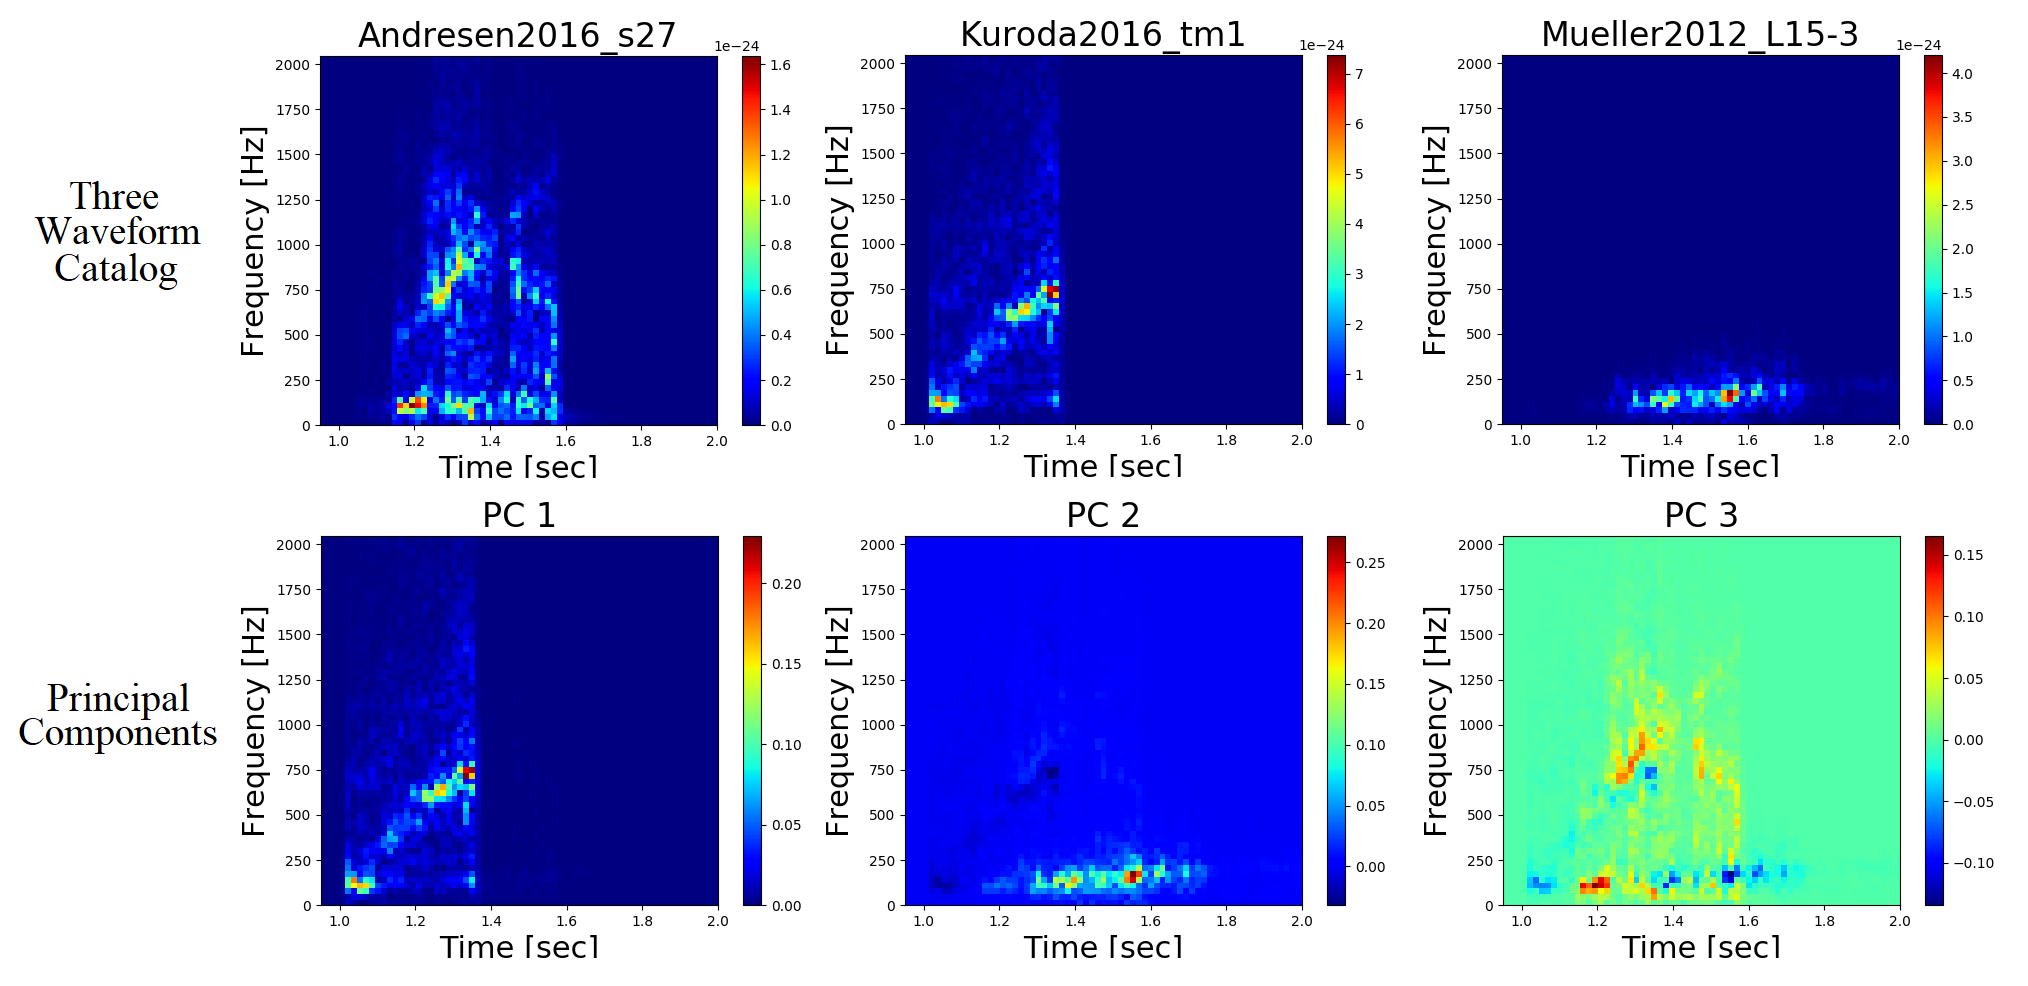
\includegraphics[width=\textwidth]{figures/PCs_example.png}
    \caption{PCs for an example catalog consisting of three neutrino model waveforms. The first PC looks very similar to the Kuroda2016\_tm1 waveform because that waveform has the largest $h_{rss}$ in this small catalog.}
    \label{fig:PCs_example}
\end{figure*}

As mentioned previously, the most important waveform features are contained in the first few PCs. In other words, PCA allows for a dimensional reduction in a data set. Catalog waveforms can usually be well-approximated with only a few PCs. The variance of the data set explained is a function of the number of PCs and is defined as~\cite{thesis_jade},
\begin{equation}
\label{equ:variance}
    v(k) = \frac{1}{\Lambda}\sum_{i=1}^{k} \Sigma_{i} \quad\text{where}\quad \Lambda = \sum_{i=1}^{n} \Sigma_{i}
\end{equation}
$\Sigma_{i}$ are the eigenvalues within $\boldsymbol\Sigma$ from equation \ref{equ:SVD}\,. Most of a catalog's variance can typically be explained by a subset of the total PCs.

A linear combination of PCs is used to construct our signal model, 
\begin{equation}
\label{equ:linear_sum}
    h_i \approx \left| \sum_{j=1}^{k} U_j \beta_j \right| \,,
\end{equation}
where $h_i$ is our reconstructed waveform (ASD spectrogram), $U_j$ is the $j$th PC, $\beta_j$ is the corresponding PC coefficient, and $k$ is the number of PCs being used. This reconstruction can then be used as a model for Bayesian model selection.

\section{Time-shifting the Signal Model} \label{sec:timeshift}

The signal model in equation \ref{equ:linear_sum} is essentially an ASD spectrogram of the signal. All of the waveforms used during the PCA are aligned in time via their times of core bounce. However, for a real CCSN signal in detector data the time of core bounce will likely not be known. Non-rotating and slowly-rotating CCSN simulations usually do not contain significant GW emission at core bounce and sometimes don't for another one or two hundred milliseconds after. Additionally, the time of arrival will be different in each detector for a multi-detector configuration. All of this means that SMEE must be able to move its signal model around in time in order to find the best reconstruction. SMEE's spectrograms contain only real data and therefore cannot be time-shifted through Fourier or similar techniques.

Our spectrograms contain 3 seconds of data and 191 individual PSDs. Each PSD is 0.03125 seconds long and has a 50\% overlap. That means the time step between subsequent PSDs is 0.015625 seconds. A spectrogram can be seen as a matrix where each column contains the PSD for a given time. The easiest way to time-shift our model is to simply shift all of our columns in one direction.  For example, shifting every column to the left by one would shift the signal model forward in time by 0.015625 seconds. The obvious concern with this method is what happens at the endpoints of the spectrogram. If we shift every column to the left by one, then the leftmost column, the first PSD, has nowhere to go. We get around this by shifting the columns in a circular fashion. If the columns are to be shifted to the left by one, then the first column would be moved to other end of the matrix to become the final column,
\begin{equation}
    \begin{bmatrix}
    1 & 4 & 7 \\
    2 & 5 & 8 \\
    3 & 6 & 9
    \end{bmatrix}
    \quad \Rightarrow \quad
    \begin{bmatrix}
    4 & 7 & 1 \\
    5 & 8 & 2 \\
    6 & 9 & 3
    \end{bmatrix}
\end{equation}
Similarly, if we were moving every column to the right by one then the rightmost column, the final column, would become the first column. We avoid issues at the endpoints by zero padding our waveforms on both sides,
\begin{equation}
    \begin{bmatrix}
    0 & 0 & 1 & 4 & 7 & 0 & 0 \\
    0 & 0 & 2 & 5 & 8 & 0 & 0 \\
    0 & 0 & 3 & 6 & 9 & 0 & 0
    \end{bmatrix}
    \quad \Rightarrow \quad
    \begin{bmatrix}
    0 & 1 & 4 & 7 & 0 & 0 & 0 \\
    0 & 2 & 5 & 8 & 0 & 0 & 0 \\
    0 & 3 & 6 & 9 & 0 & 0 & 0
    \end{bmatrix}
\end{equation}
All of our waveforms are aligned with their core bounces at t = 1 second. None of our waveforms are longer than 1.5 seconds, which means that every signal model reconstruction has at least 0.5 seconds of zero padding at the end. All of this together means that we can perform a circular time-shift up to 0.5 seconds in either direction without issues. For a real signal then, our estimated core bounce time must be within a half second of the actual core bounce time, which is very feasible. If we wanted to time-shift by more than 0.5 seconds we could simply increase the amount of zero padding. Lengthening our spectrograms from 3 to 4 seconds for example, would allow for 1 second time-shifts in either direction.

The main detriment to this method is the simple fact that our temporal resolution is limited to 0.015625 seconds. While this is not ideal, it is significantly shorter than typical CCSN waveforms and has not been a concern in testing.

\section{Priors}
\label{sec:priors}

The evidence in equation \ref{equ:evidence_def} for a given signal model depends on the following parameters: time (arrival at Earth geocenter), source position (right ascension, declination, and polarization angle), $h_{rss}$\,, and the PC coefficients in equation \ref{equ:linear_sum}\,. The number of PCs, and coefficients, is optional. After running SMEE to produce a Bayes factor, posterior distributions can be created for each parameter listed. In many situations the sky location will be known, in which case the right ascension and declination parameters will be constants obtained from astronomers.

SMEE's algorithm is initiated with an estimated arrival time chosen by the user. As discussed in the previous section, SMEE can time-shift its signal models 0.5 seconds in either direction. The prior distribution for time is then bounded 0.5 seconds before and after the estimated arrival time and has a flat (uniform) shape. When the sky position is unknown, right ascension is bounded between $[0, 2\pi]$ with a flat shape and declination is bounded between $[-\frac{\pi}{2}, \frac{\pi}{2}]$ with its shape uniform in cosine. The source polarization angle is always bounded between $[0, \pi]$ with a flat shape. The upper and lower bounds on $h_{rss}$ can be chosen by the user and the prior is uniform in volume. If the chosen lower bound is too small, then SMEE will always return $\log B_{S,N} \approx 0$ as the signal and noise models are statistically indistinguishable. The upper bound on $h_{rss}$ can be freely chosen as long as it is above the actual value.

The remaining parameters are the PC coefficients, all of which have flat, uniform priors. The upper and lower bounds for these can be determined in various ways, including simple experimentation. This process results in wider bounds for the first few PCs as they are typically more heavily used (have larger coefficients) in reconstructions. A more targeted approach is to calculate the dot product between each PC and each catalog waveform~\cite{thesis_josh, thesis_jade, heng:09}. Doing this will give the coefficients needed to reconstruct each catalog waveform out of the PCs. Once all of the these coefficients are known, the catalog minimum and maximum values can be found for each PC coefficient. The upper and lower prior bounds can then be set to these values plus or minus $\sim 10\%$\,. This gives bounds that are based upon the catalog waveforms but account for some simulation uncertainty.

\section{Nested Sampling}

In order to perform Bayesian model selection, SMEE must calculate the evidence integral in equation \ref{equ:evidence_def}\,. To do this, SMEE uses the LALInference Nested Sampling algorithm within LIGO's Algorithm Library (LAL)~\cite{thesis_jade, veitch:15}. Nested Sampling is a numerical technique that can solve evidence integrals and produce posterior distributions for the parameters of a model~\cite{thesis_josh}. The evidence can be written as,
\begin{equation}
\label{equ:evidence_algrebra}
    \begin{split}
    Z =& \int_{\theta} p(\theta|M)p(D|\theta,M)d\theta \\
    \approx& \sum_{i=1} p(D|\theta_{i},M)\omega_{i} \\
    \approx& \sum_{i=1} \mathcal{L}_{i}\omega_{i} \\
    \end{split}
\end{equation}
where $\omega_{i}$ is the weight, indicating the fraction of the prior distribution represented by the $i$th sample, and $\mathcal{L}_{i} = p(D|\theta_{i},M)$ is the likelihood. Initially, a set of data points is randomly chosen from the prior. Each of these ``live points" represent a possible waveform reconstruction and have likelihood values associated with them. The point with the lowest likelihood will have the largest prior mass, where prior mass, $X$, is defined,
\begin{equation}
\label{equ_prior_mass}
    X(\nu) = \int_{\mathcal{L}(\theta)>\nu} p(\theta|M)d\theta
\end{equation}
$\nu$ represents a likelihood value in the formula above. As $\nu$ increases, the prior mass, $X\,$, decreases. Each iteration of the nested sampling, the point with the lowest likelihood and largest prior mass will be replaced. The likelihood and prior mass values for that point are then used as limiting values for the replacement live point. This new live point is generated within those limiting values using Markov Chain Monte Carlo techniques~\cite{sivia1996data, thesis_jade}. This repeats with the live points iteratively converging upon the region of the prior with the highest likelihood. Figure \ref{fig:nested_sampling} illustrates this procedure. When a signal is present, the evidence integral will be dominated by this small region of the prior. This high likelihood region of the prior is concentrated in a fraction, $e^{H}$, of the parameter space. $H$ is referred to as the information in the data, and is defined,
\begin{equation}
    \begin{split}
    H =& \int \log \frac{dP}{dX}dP \\
    \approx& \sum p(\theta|D,M)\log\frac{p(\theta|D,M)}{dX} d\theta
    \end{split}
\end{equation}
\begin{figure*}[t!]
    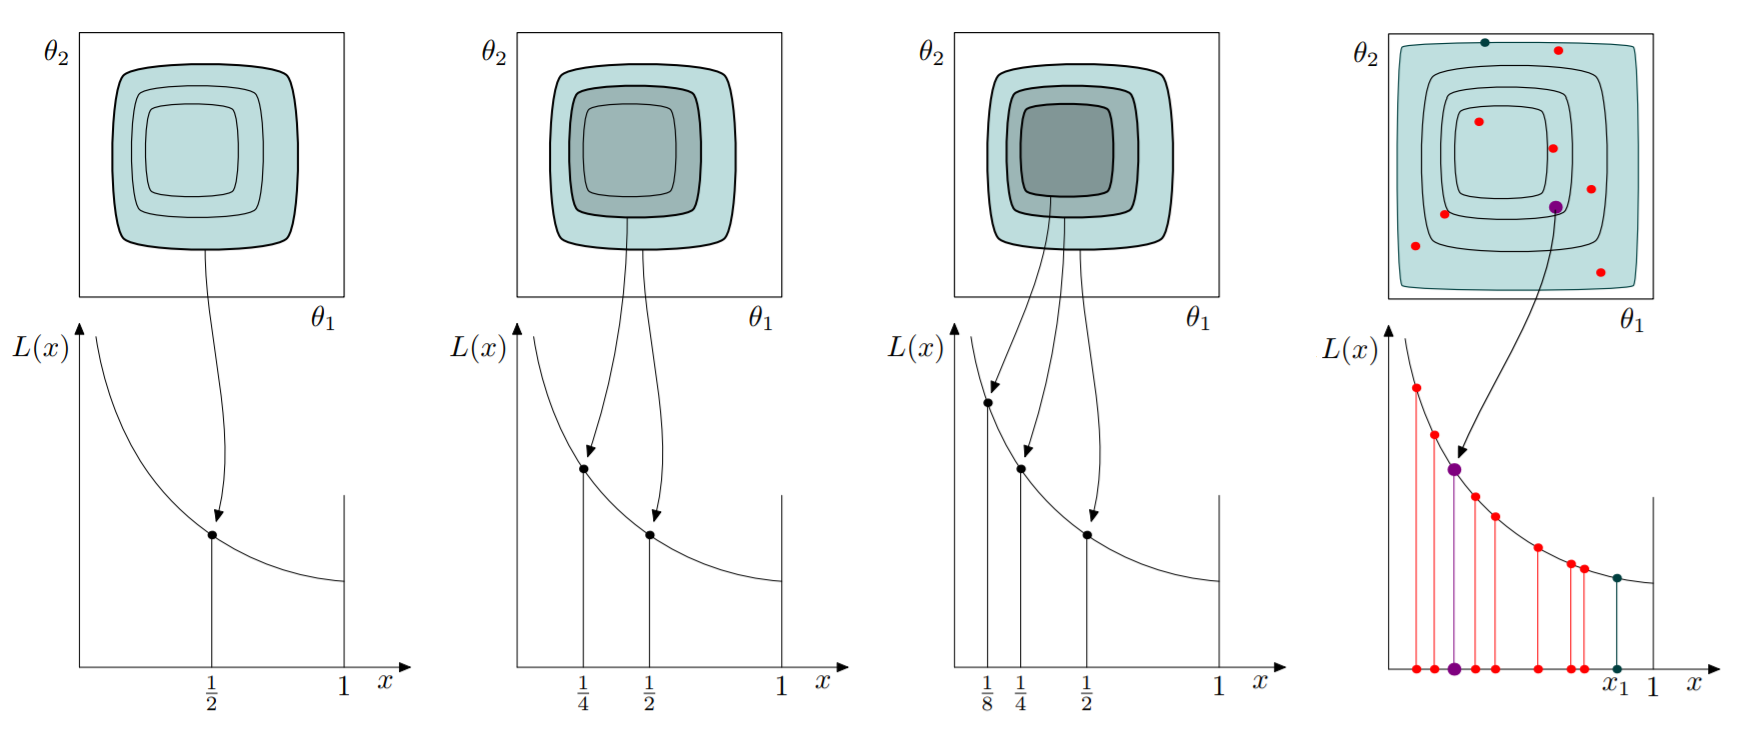
\includegraphics[width=\textwidth]{figures/nested_sampling.png}
    \caption{A visualization of the nested sampling algorithm. Plots along the top represent contour plots of a likelihood function. Bottom plots show likelihood, $L(x)$\,, vs prior mass, $x$. Initially, points are selected uniformly from the prior. Points with the largest likelihoods enclose the smallest prior masses. During each iteration of the sampling, the point with the lowest likelihood ($x_{1}$ in rightmost plot) is replaced via MCMC by a new point uniformly distributed between $0$ and $x_{1}$\,. This shrinks the prior mass and converges upon the best solution. Plots reproduced from \cite{nested_sampling}.}
    \label{fig:nested_sampling}
\end{figure*}
where $P$ represents the posterior mass. $H$ can be said to represent the amount of information in the posterior relative to the prior. Eventually, the likelihoods of the live points will be maximized and each iteration of the nested sampling will provide minimal improvement. At this point the evidence has been sufficiently calculated and the sampling must stop. This is implemented in the code as a cutoff when $i > mH\,$, where $i$ is the number of iterations, $m$ is the number of live points, and $H$ is the information. When this point is reached, the signal and noise evidences have been calculated and SMEE outputs its final result, a signal vs. noise Bayes factor,
\begin{equation}
    \begin{split}
    \log B_{S,N} =& \log[p(D|M_{S})] - \log[p(D|M_{N})] \\
    =& \log Z_{S} - \log Z_{N}
    \end{split}
\end{equation}

After running SMEE with two different sets of PCs, we will have two Bayes factors, each representing a model. A final Bayes factor comparing these two models can be constructed with simple subtraction,
\begin{equation}
\label{equ:model_selection}
    \begin{split}
    \log B_{S_{1},S_{2}} =& \log B_{S_{1},N} - \log B_{S_{2},N} \\
    =& (\log Z_{S_{1}} - \log Z_{N}) - (\log Z_{S_{2}} - \log Z_{N}) \\
    =& \log Z_{S_{1}} - \log Z_{S_{2}}
    \end{split}
\end{equation}
When $\log B_{S_{1},S_{2}} > 0\,$, model $S_{1}$ is preferred, and when $\log B_{S_{1},S_{2}} < 0\,$, model $S_{2}$ is preferred. A confidence threshold, $C\,$, will typically be set on the final Bayes factor. When,
\begin{equation}
\label{equ:confidence_threshold}
    \left|\log B_{S_{1},S_{2}}\right| \geq C
\end{equation}
then the preferred model can be selected with confidence. A reliable confidence threshold can be determined through experimentation, but typical values are in the range of 3-10\,.

\section{Posterior Distributions}

\begin{figure*}[p]
    \centering
    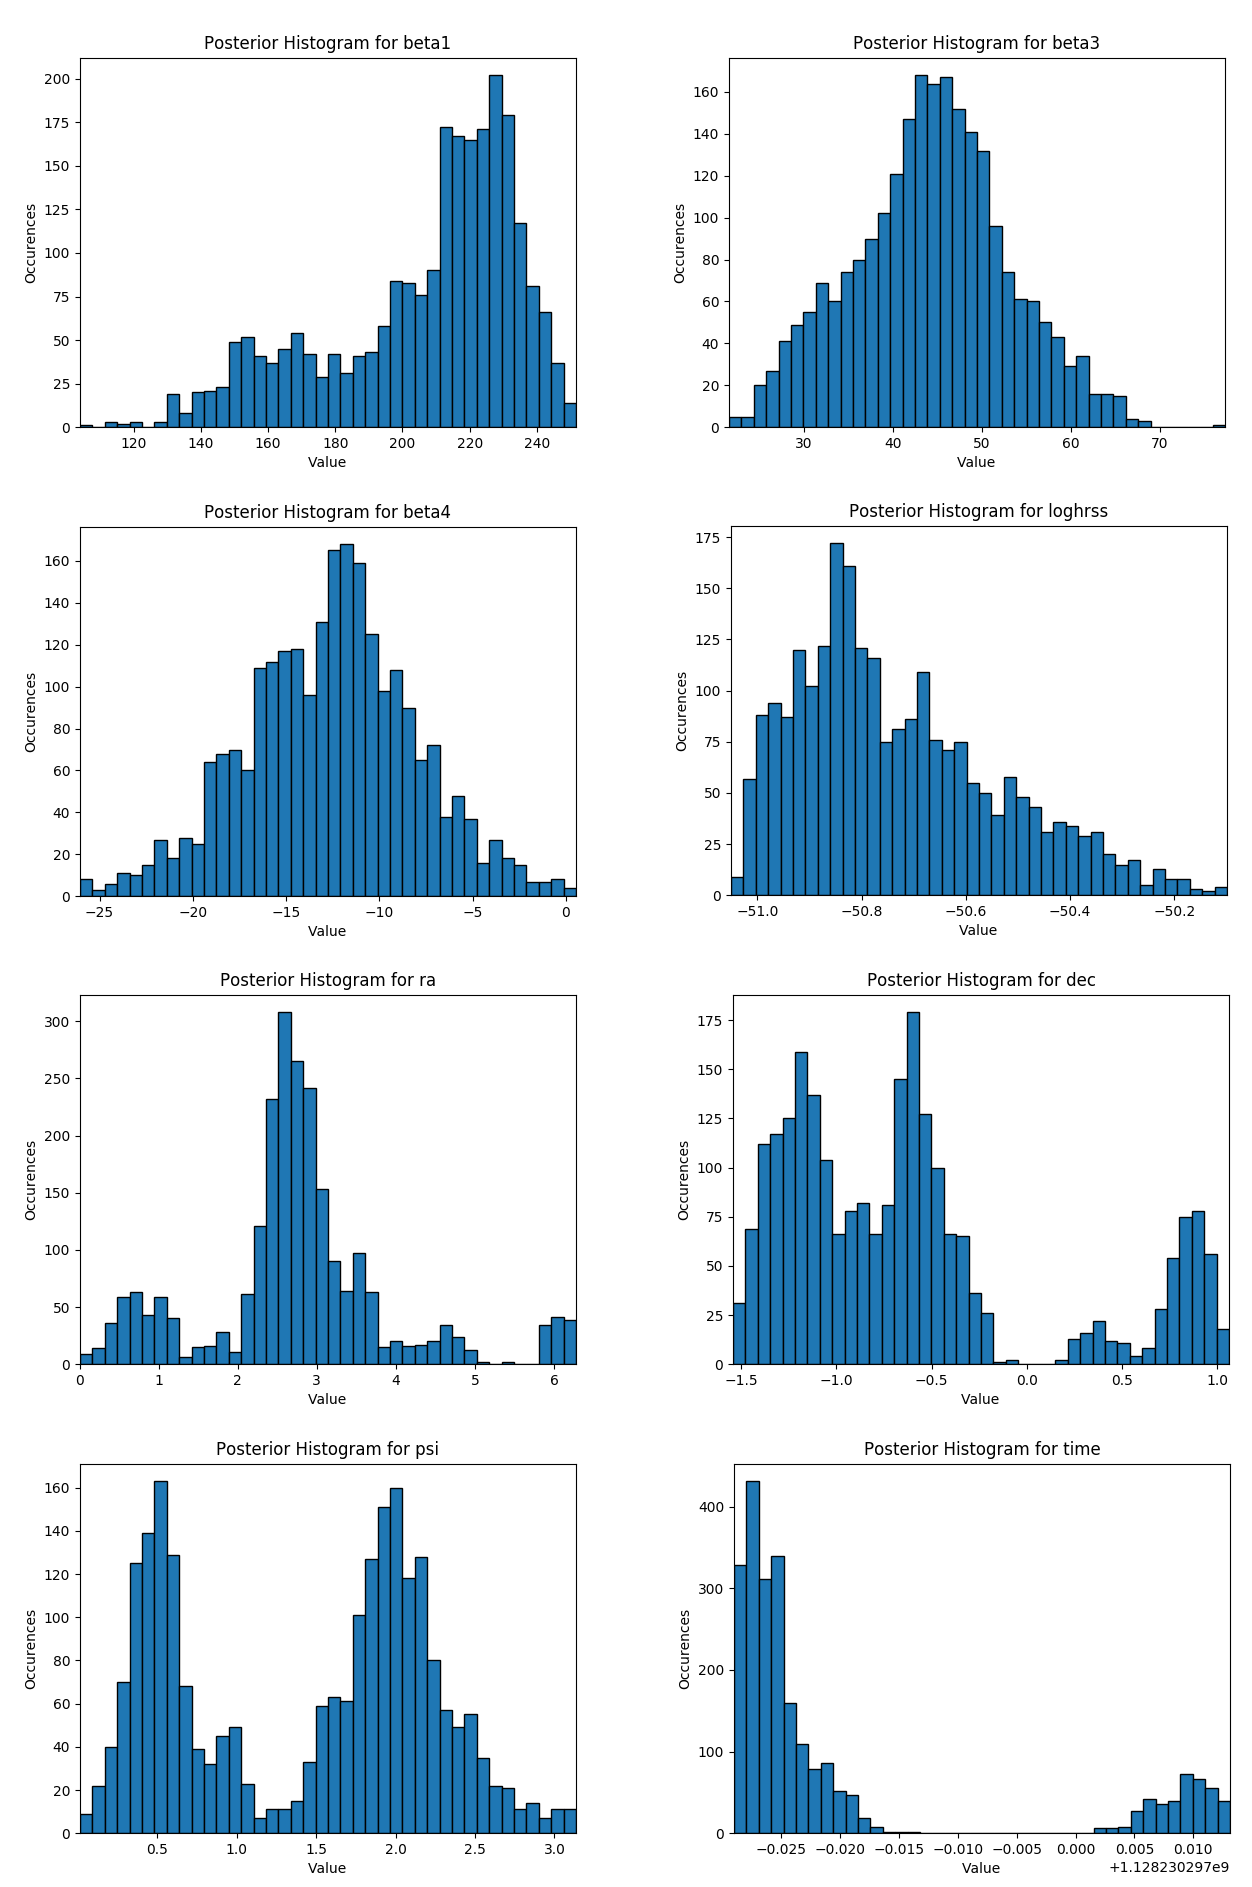
\includegraphics[width=5.1in]{figures/posteriors.png}
    \caption{Posterior distributions for a sample of SMEE's parameters. Betas refer to PC coefficients. Sky localization, represented by right-ascension (ra), declination (dec), and psi, is limited by the fact that SMEE only reconstructs one GW polarization. For most CCSN it is expected that the sky position will be known.}
    \label{fig:posteriors}
\end{figure*}

The Bayes factor is the primary output of SMEE, but a posterior distribution is also produced for each parameter. These parameters include the PC coefficients, the signal $h_{rss}$, the arrival time (center earth), and the sky position. When producing a reconstruction, the maximum likelihood data point is used. This is the last data point produced during nested sampling, as shown in Figure~\ref{fig:nested_sampling}.

Figure~\ref{fig:posteriors} contains example posterior distributions for an injected CCSN waveform. It is possible for SMEE to determine the sky location when not previously known, but the effectiveness of this is somewhat limited by the fact that SMEE only reconstructs one polarization of the signal. For most CCSN signals it is expected that a sky location will be known through electromagnetic and neutrino observations.

\section{Signal Model Catalogs}

\begin{figure*}[p]
    \centering
    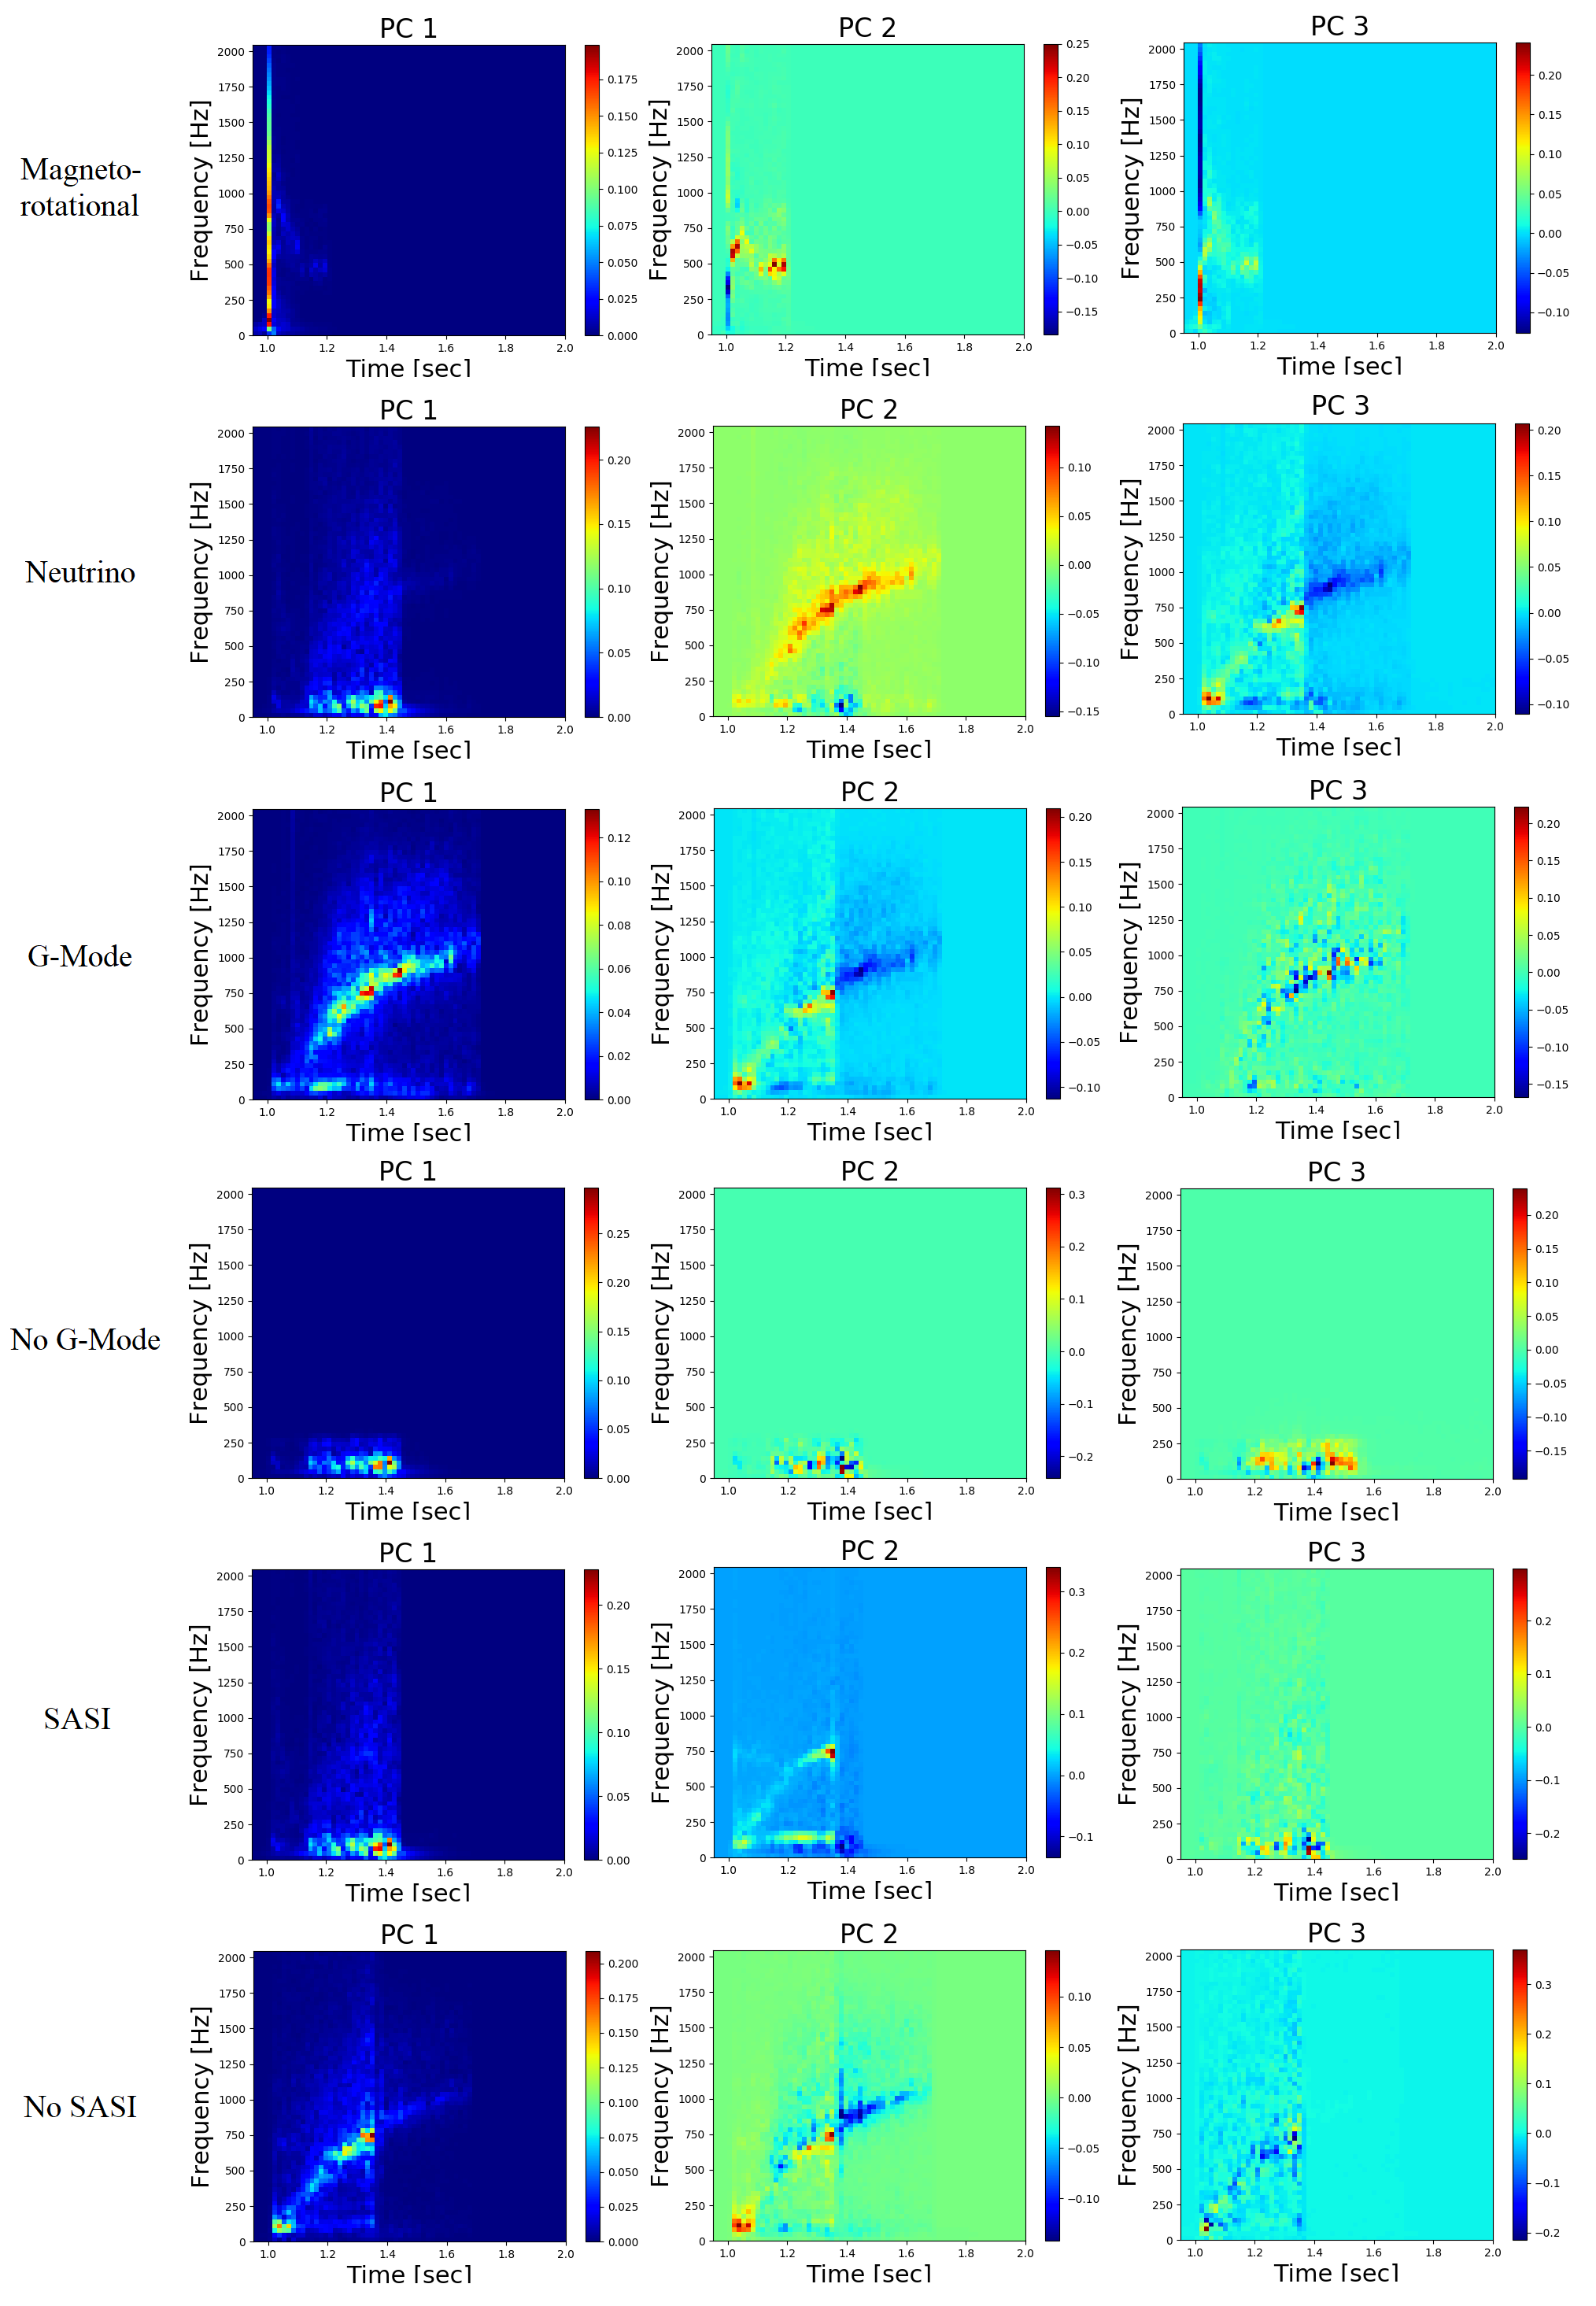
\includegraphics[width=5.5in]{figures/all_PCs.png}
    \caption{The first three PCs for each catalog. From top to bottom, the catalogs are: neutrino mechanism, magnetorotational mechanism, g-modes, no g-modes, SASI, and no SASI. Two catalogs are compared to each other for each classification statement.}
    \label{fig:all_PCs}
\end{figure*}

The first classification statement that SMEE makes is a determination of the explosion mechanism. After core bounce, the stalled shock front must be re-energized in order to successfully cause a supernova explosion. As described in section~\ref{sec:mechanisms}, simulation groups have settled upon two main models to explain this re-energization, the neutrino model for non or slowly-rotating progenitors~\cite{mueller:e12, kuroda:16, andresen:16}, and the magnetorotational model for rapidly-rotating progenitors~\cite{scheidegger:10b, scheidegger2010gravitational}. A signal catalog can be constructed for each model with waveforms of that type. These catalog waveforms will typically come from multiple simulation groups. Each signal catalog produces a set of PCs (as seen in Figure \ref{fig:all_PCs}) that can then be used with SMEE to produce a signal vs noise Bayes factor. Those Bayes factors can then be compared to each other via subtraction to produce a final signal model vs signal model Bayes factor, as in equation \ref{equ:model_selection}. This result tells us which explosion mechanism is more likely for the observed CCSN signal.

The other two classification statements that SMEE makes are related to the presence of predicted features (SASI and g-modes) in the GW signal. As described above, in order to make a statement about the CCSN re-energization mechanism two different sets of PCs had to be used. Each set corresponds to a signal model and the two resulting Bayes factors can then be compared. We follow a similar procedure for waveform feature statements, with one catalog consisting of waveforms that possess the feature and one catalog consisting of waveforms that do not possess the feature (as seen in Figure \ref{fig:all_PCs}). The ``g-mode" Bayes factor, for example, can then be compared to the ``no g-mode" Bayes factor to determine whether g-modes appear to be present in the signal. The procedure is identical for SASI. It should be noted that only neutrino model waveforms are used in these waveform feature catalogs. These features are usually less prominent in rapidly-rotating simulations as the tremendous rotation can suppress convective motion~\cite{2016arXiv160501785A, scheidegger:10b}. Because all of these waveforms are neutrino model waveforms, the performance difference between competing signal model reconstructions can be subtle. Low SNR situations in which only part of the signal is detectable can also be problematic as waveform features can be lost in the noise. This can lead to a higher confidence threshold in equation \ref{equ:confidence_threshold} to ensure good performance for quiet signals.

\section{Number of Principal Components}

\begin{figure*}[t!]
    \centering
    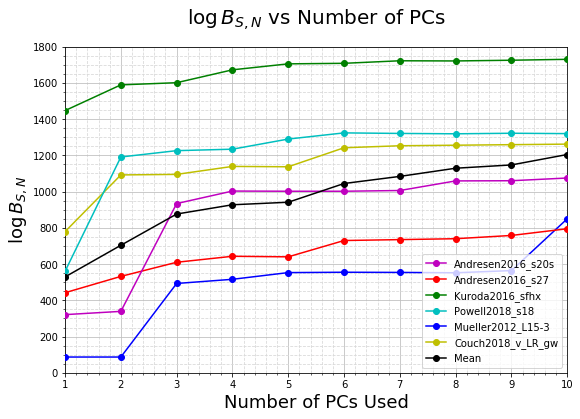
\includegraphics[width=2.9in]{figures/PCs_neu_review.png}
    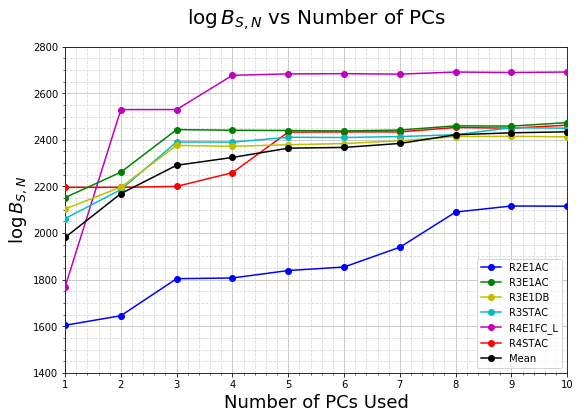
\includegraphics[width=2.9in]{figures/PCs_sch_review.png}
    \caption{Log Bayes factors for mechanism classification with an increasing number of PCs in simulated aLIGO Gaussian noise. Waveforms with a * were not included when making the PCs. The left figure shows neutrino catalog waveforms, and the right figure shows magnetorotational catalog waveforms. 6 PCs for the neutrino model and 5 for the magnetorotational model would be acceptable choices as there is limited $\log B_{S,N}$ improvement beyond those points.}
\label{fig:pick_pcs}
\end{figure*}

The number of PCs used can vary within SMEE. In general, the reconstructions will improve at a diminishing rate as more PCs are included. Figure~\ref{fig:pick_pcs} shows this for mechanism classification PCs. Naturally it is desirable to find a number of PCs that can sufficiently reconstruct every catalog waveform, but Bayesian inference tends to prefer simpler models, especially in low SNR cases, due to the Occam factor~\cite{mackay2003information, thesis_jade}. Models with large numbers of parameters can predict a larger number of data sets and the confidence of individual results suffers a penalty. Figure~\ref{fig:pick_pcs} was produced by injecting CCSN waveforms into Gaussian data with an SNR of 20. The number of PCs can also be chosen by setting a threshold on the explained variance, defined in equation~\ref{equ:variance}.